% -*- coding: utf-8 -*-
\documentclass[12pt,openright]{book}

\usepackage{ifxetex}
\ifxetex
  \usepackage[bookmarksnumbered]{hyperref}
\else
  \usepackage[unicode,bookmarksnumbered]{hyperref}
\fi

\usepackage[emptydoublepage]{NKThesis}   % 中文

%   根据需要选择 biblatex 宏包选项.
\usepackage[backend = biber, defernumbers = true,  sorting=none,  style = nkthesis]{biblatex}
\hypersetup{colorlinks=true,
            pdfborder=0 0 1,
            citecolor=black,
            linkcolor=black}
\usepackage{tikz}
\usepackage{bm}
\usepackage{caption}
\usepackage{graphicx, subfig}
\usepackage{fontspec}
\usepackage{listings}
\usepackage{xcolor}
\setmonofont{Consolas}
% 定义可能使用到的颜色
\definecolor{CPPLight}  {HTML} {686868}
\definecolor{CPPSteel}  {HTML} {888888}
\definecolor{CPPDark}   {HTML} {262626}
\definecolor{CPPBlue}   {HTML} {4172A3}
\definecolor{CPPGreen}  {HTML} {487818}
\definecolor{CPPBrown}  {HTML} {A07040}
\definecolor{CPPRed}    {HTML} {AD4D3A}
\definecolor{CPPViolet} {HTML} {7040A0}
\definecolor{CPPGray}  {HTML} {B8B8B8}
\lstset{
    columns=fixed,       
    numbers=left,                                        % 在左侧显示行号
    frame=none,                                          % 不显示背景边框
    backgroundcolor=\color[RGB]{245,245,244},            % 设定背景颜色
    keywordstyle=\color[RGB]{40,40,255},                 % 设定关键字颜色
    numberstyle=\footnotesize\color{darkgray},           % 设定行号格式
    commentstyle=\it\color[RGB]{0,96,96},                % 设置代码注释的格式
    stringstyle=\rmfamily\slshape\color[RGB]{128,0,0},   % 设置字符串格式
    showstringspaces=false,                              % 不显示字符串中的空格
    language=c++,                                        % 设置语言
    morekeywords={alignas,continute,friend,register,true,alignof,decltype,goto,
    reinterpret_cast,try,asm,defult,if,return,typedef,auto,delete,inline,short,
    typeid,bool,do,int,signed,typename,break,double,long,sizeof,union,case,
    dynamic_cast,mutable,static,unsigned,catch,else,namespace,static_assert,using,
    char,enum,new,static_cast,virtual,char16_t,char32_t,explict,noexcept,struct,
    void,export,nullptr,switch,volatile,class,extern,operator,template,wchar_t,
    const,false,private,this,while,constexpr,float,protected,thread_local,
    const_cast,for,public,throw,std},
    emph={map,set,multimap,multiset,unordered_map,unordered_set,
    unordered_multiset,unordered_multimap,vector,string,list,deque,
    array,stack,forwared_list,iostream,memory,shared_ptr,unique_ptr,
    random,bitset,ostream,istream,cout,cin,endl,move,default_random_engine,
    uniform_int_distribution,iterator,algorithm,functional,bing,numeric,},
    emphstyle=\color{CPPViolet}, 
}

\addbibresource{nkthesis.bib}
\DeclareBibliographyCategory{cited}
\AtEveryCitekey{\addtocategory{cited}{\thefield{entrykey}}}

\title{一种高效的多物理场动力学模拟方案\footnote{项目托管于\url{https://github.com/NKUCSPaperGroup/KinematicsSimulation}}}
\author{周子正\footnote{学号:1810334,电子邮箱:zhouzizheng@foxmail.com},刘雨缇\footnote{学号:1811495},周宇江\footnote{学号:1810333},张轩珩\footnote{学号:1810320}}
\date{2018年 12月}

\begin{document}
\maketitle
% -*- coding: utf-8 -*-
\begin{zhaiyao}
质点动力学问题是最常见的动力学问题,本文以场和质点为基本单位,提出了一套方法并实现了一个c++库,可以概括性的解决所有此类问题,
并提出了碰撞处理的一种新的手段。在解决问题的同时,将精度提高到四阶,将时间消耗降至最小。并且能高度并行,有很好的可拓展性。


例如,二体问题,三体问题,各类碰撞问题,复杂电磁场下的运动问题,都是此问题的简单子集。
\end{zhaiyao}


\begin{guanjianci}
质点动力学,高性能,碰撞处理,并行化,八叉树
\end{guanjianci}



\begin{abstract}
    Particle dynamics is the most common dynamic problem. In this paper which uses the field and particle as the basic unit, a set of methods and a c++ library are proposed and implemented, which can solve the problems above in a general way. Also, a new method of collision processing is created. By this means,the accuracy is improved to the fourth order and the time consumption is minimized. In addition, it can be highly parallel, and has a good scalability.
    

    For example, two-body problem, three-body problem, various collision problems, and motion problems under complex electromagnetic fields are all simple subsets of this problem.    
\end{abstract}


\begin{keywords}
Particle dynamics, High performance, Collision processing, Parallelization, Octree
\end{keywords}

\tableofcontents
%!TEX program = xelatex
% -*- coding: utf-8 -*-
\chapter{引言}
\section{设计背景}
质点动力学问题是动力学问题的基础,动力学是物理学和天文学的基础,也是许多工程学科的基础。许多数学上的进展也常与解决动力学问题有关.
而一切质点之间都应该通过内力或者外力进行相互作用,质点对力的反应都遵循相似的规律,力的作用也遵循某种确定的规律。
因为质点的动力学问题包含着某种普遍性。


质点动力学有两类基本问题:一是已知貭点的运动,求作用于质点上的力,二是已知作用于质点上的力,
求质点的运动,求解第一类问题时只要对质点的运动方程取二阶导数,得到质点的加速度,代入牛顿第二定律,即可直接求得力,不在此赘述;
求解第二类问题时需要求解质点运动微分方程。


通常情况下我们使用微分方程求解动力学问题,尽管这是一种成熟的方法,但在目前所研究的力学系统中,需要考虑的因素逐渐增多,
例如,变质量、非线性、非保守还加上反馈控制、随机因素,同时物体的数量极大等,变元的个数迅速增长,方程的形式非常复杂,
这使运动微分方程越来越复杂,可直接求解的问题越来越少,许多动力学问题都需要用数值计算法近似地求解


但是数值近似的方法往往需要首先对在复杂场景中的大量物体进行逐个分析,高度耦合的场景和大量的物体使得这个过程很难进行,
当物体的数量相当多,方程形式足够复杂时,试图完备的分析每一个质点几乎是不可能的。
我们试图采取一种相反的手段,将自上而下构造方程的过程抽象,转而由边界条件迭代的给出状态解。
这样模拟式的设计使得我们可以只独立的考虑某一个场或物体,在修改它的时候不需要修改方程,简化分析过程。


在一般的模拟方法中,由于状态突变产生的奇点,由于物体数量过大产生的高复杂度分别从计算的精度和计算的时间上制约着模拟方法的应用,
我们试图通过几种模型简化计算的数量,同时提高计算的精度。


\section{解决的问题}
经典的二体问题和三体问题是质点系动力学中的经典问题。此类N体问题,都可以被此框架解决。
多体碰撞问题,大空间尺度上的宇宙动力学问题,复杂电磁场下的运动问题,也都是此问题的子集。

正如上面所提到的,这个库可以求解多质点场景下的多物理场作用,同时可以考虑内部相互作用。

在这个库中,物理场可以完全自定义。同时,我们致力于优化求解方案,使得速度提高,精确度提高。为使计算能够适应大规模集群计算的场景,我们设计了高度并行化的计算方案。

在下面的讨论中,我们讲解释如何普适的解决动力学问题,并如何将这一过程抽象。

\newpage

\section{理论基础}

\subsection{动力学理论基础}
\subsubsection{对物理学部分的分析}
\noindent 
考虑质点系中的某一个质点$i$,由牛顿第二定律有
\[
    m_{i}\bm{a}_i = \sum_{p=1}^{M}{\bm{F}_p} + \sum_{i \neq j } \bm{f}_{ij}
\]
根据运动学原理,有
\[
    \left\{
        \begin{array}{l}
            {\displaystyle \bm{v} = \frac{d\bm{r}}{dt}}\\
            \\
            {\displaystyle \bm{a} = \frac{d\bm{v}}{dt}}
        \end{array}
    \right.
\]


可以看到力是物体运动的直接原因,所以只需要给出正确的力的作用即可计算出物体的运动。

对于任意的外力,总可以考虑成一种场的作用,即$F = F(t,\bm{r})$。

对于任意的内力,总可以考虑为一种附着在物体上的场的作用。

综合上述的叙述,由场作为力源实体,力作为作用的传递方式,质点作为运动对象的形式可以普适的解决动力学问题。

\subsubsection{对数学部分的分析}
对于一个连续的动力学问题,我们可以将其离散化。最简单的是利用欧拉法。不失一般性,我们讨论一个质点的计算。

\[
    \left\{
        \begin{array}{l}
            {\displaystyle m\bm{a}_{n} = \bm{F}_{sum}(t_n,\bm{r}_n)}
            \\
            {\displaystyle \bm{v}_{n+1} = \bm{v}_{n} + \Delta t a_n }
            \\
            {\displaystyle \bm{r}_{n+1} = \bm{r}_{n} + \Delta t v_n  }
            \\
            {\displaystyle t_{n+1} = t_n + \Delta t}
        \end{array}
    \right.
\]\label{eular}

我们可以通过对任意$t$时刻的状态的计算得到$t+\Delta t$时刻的状态,从而迭代的完成了对全过程的计算。

\subsection{对碰撞的特殊处理}
在计算的过程中,碰撞的处理是一个难点,如果不能将碰撞的情况对称的纳入到现有的计算框架,将会使得运动方程在碰撞出出现奇点。
为解决这个问题,我们考虑将碰撞转化为力场。


我们构造这样的一种力,它在一个很短的时间(但大于计算的步长)上的作用结果正好是碰撞本身产生的瞬时冲量的结果。
显然,在计算的步长和碰撞力(我们暂且这么称这种力)的作用时间同时趋于0的时候,结果就是瞬时碰撞产生的结果。
由于碰撞是一种相互的作用,它满足牛顿第三定律 $ F_ij = -F_ji $ 。
根据经典力学,碰撞的冲量是:

\[
    I = mv_t - mv_0
\]

其中,$v_t,v_0 $ 可以通过方程组解得

\[
    \left\{
    \begin{array}{l}
        {\displaystyle m_1 \bm{v}_{10} + m_2 \bm{v}_{20} = m_1\bm{v}_{1t}+m_2\bm{v}_{2t} }
        \\
        {\bm{v}_{1t}-\bm{v}_{2t} = e(\bm{v}_{10}-\bm{v}_{20})}
    \end{array}
    \right.
\]

得到$ I $后,一种最简单的手段构造这种力是另其在这个区间上的分布是相同的,即力在这段时间上的导数是$0$。由此可得
\[ \bm{F}_{collide} = \frac{I}{ \Delta t} \]

联立上述的方程,可以计算得到 $\bm{F}_{collide} $,将碰撞这一过程转化为了受力的过程。
在解决碰撞奇点的同时,此转化方法还能够解决三体碰撞问题,由于力的可加性,多体的碰撞效果可以相互叠加得到正确的状态,在此处不做赘述。

\chapter{项目的设计}
我们将采用c++语言描述设计,设计不依赖于语言,可以简单的移植到其他平台。
\section{项目的架构}
可以看到,物体的速度,位置,加速度,力等都是一个向量。所以首先我们应该对物理计算中大量出现的向量进行统一控制,我们将其设计为了值类型。
由于向量在坐标变换中的不变性,所以不失一般性,我们将向量定义在空间直角系中,以三个参量表示,并实现向量的基本计算接口。\\
对在动力学系统中传递作用的力,我们特化建立一个新的类型,并且在描述一个力矢量性的同时描述它的类型。如\ref{cd1}所示

\begin{figure} 
    \centering 
    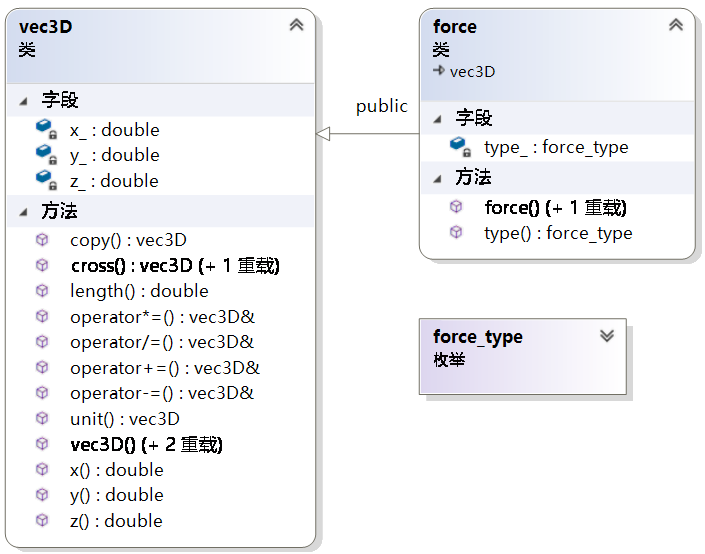
\includegraphics[width=.8\textwidth]{ClassDiagram1.png}
\caption{vec3D和force的架构} %caption是图片的标题 
\label{cd1} %此处的label相当于一个图片的专属标志,目的是方便上下文的引用 
\end{figure}

我们将物体的几何部分抽象成一个类,它表示成一个长方体,作为物体的包装盒,物体应该完全存在于这个包装盒中,
我们实现了这个类的碰撞检测,它能够在 $ O(1) $ 的时间内快速的完成,作为一种最粗糙的检测。


质点和场都继承自这个类,以进行物体实体在空间中的统一管理。
field类内的两个纯虚函数表示对场的边界
\footnote{对于任何的一个物体,场总会给出它是否在场内,这样其实概括性的定义了一个范围,即$ \{(x,y,z)|F(x,y,z)=1\} $}
和场的描述
质点中实现了对受力的反应,能够在每次更新的时候根据当前受力进行移动,如\ref{cd2}和\ref{cd31}所示

\begin{figure} 
    \centering 
    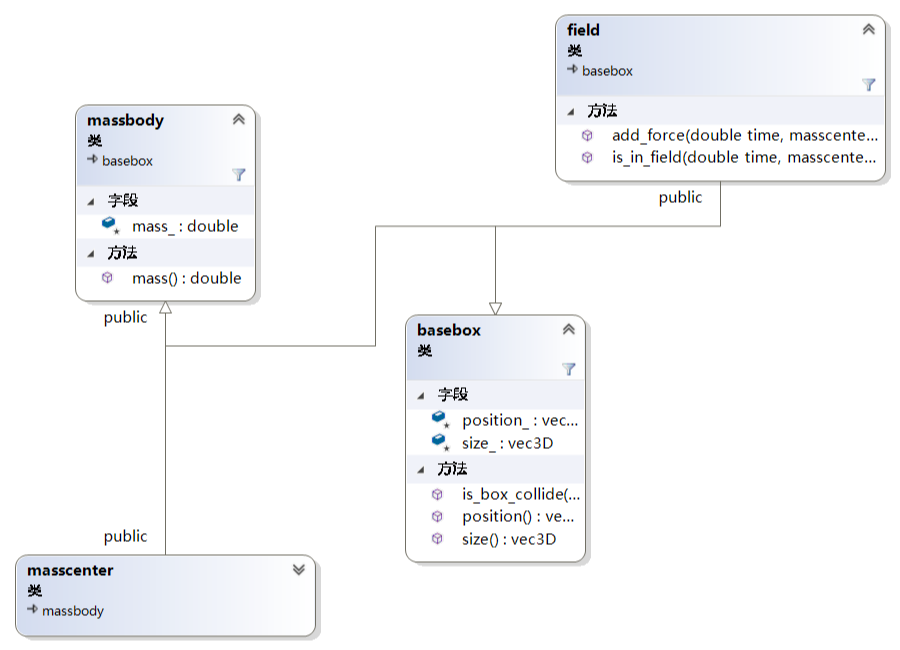
\includegraphics[width=.9\textwidth]{ClassDiagram2.png}
\caption{masscenter和field的架构} %caption是图片的标题 
\label{cd2} %此处的label相当于一个图片的专属标志,目的是方便上下文的引用 
\end{figure}

\begin{figure} 
    \centering 
    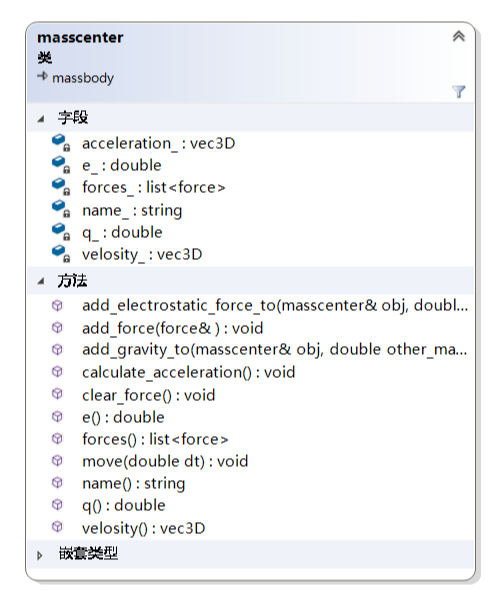
\includegraphics[width=.8\textwidth]{ClassDiagram31.png}
\caption{masscenter的实现细节} %caption是图片的标题 
\label{cd31} %此处的label相当于一个图片的专属标志,目的是方便上下文的引用 
\end{figure}

为了对质点和场的作用以及质点之间相互作用的情况进行统一计算,一个管理对象的容器类是必要的,这种设计使得物体只代表它的状态,不代表它的计算,将组合多种对象的计算从某种对象中剥离出来,
实现更好的解耦。由于管理的对象可以被扩展,比如抽象类field内两个方法的不同实现可以表示完全不同的场,场的性质具有多样性,而对场的计算又有统一性,通过容器的管理可以只调用被管理对象的相关接口。
只对接口的调用满足了计算的统一性,field的多态实现又满足了场的性质的多样性,这样程序在完成计算逻辑的同时完全符合开闭原则\footnote{对修改关闭,对拓展开放}。

\begin{figure} 
    \centering 
    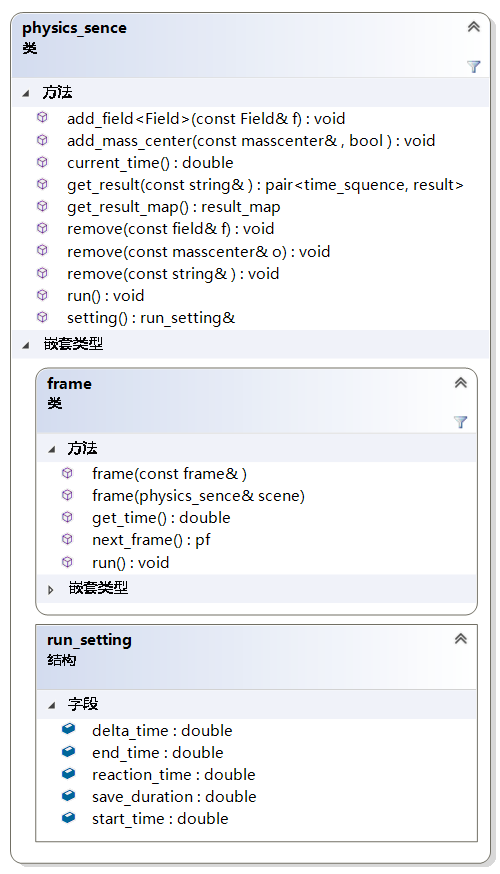
\includegraphics[width=.7\textwidth]{ClassDiagram3.png}
\caption{physics\_scene的架构} %caption是图片的标题 
\label{cd3} %此处的label相当于一个图片的专属标志,目的是方便上下文的引用 
\end{figure}

最后,设计了一个类在程序运行的同时自动地记录感兴趣的数据。如\ref{cd5}所示

\begin{figure} 
    \centering 
    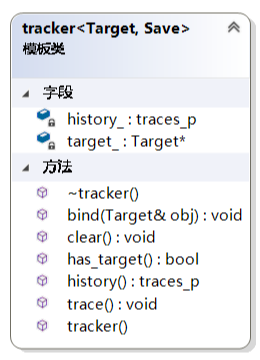
\includegraphics[width=.4\textwidth]{ClassDiagram5.png}
\caption{tracker的架构} %caption是图片的标题 
\label{cd5} %此处的label相当于一个图片的专属标志,目的是方便上下文的引用 
\end{figure}

整个结构的运行是按照如下的顺序进行的:
\begin{enumerate}
    \item 构造masscenter对象描述初态
    \item 构造field对象描述物理场
    \item 构造physics\_scene对象描述求解问题的范围与精度设置
    \item 将两种物理对象加入到物理场景中
    \item 运行这个场景
    \item 得到追踪的对象在每一个时刻的状态
    \item 导出计算结果并进行分析
\end{enumerate}

\section{对速度的优化}
\subsection{八叉树的引入}
在计算的过程中,对时间消耗最大的是碰撞检测的具体细节以及对碰撞之后的结果的计算。事实上,质点与场之间的作用可以理解为质点和与质点碰撞的场的运动。
在常规计算中,碰撞检测基于一种轮询,其时间复杂度为$O(n^2)$这个结果在$n$很大的时候并不高效。考虑到并不是在一个空间的物体就会发生碰撞,我们以一种更好的结构管理空间中的对象,使得碰撞检测的复杂度下降。

首先我们考虑一个简单的例子,在一个直线上的线段相交的检测。考虑如果一个线段和另一个线段分别位于一个点的两侧时,这两个线段不可能相交。
我们在直线上选取一个合适的点并在此处将这条线段一分为二,这样这个直线就变成了两个部分,如果直线的长度本身是有限的,这个过程会生成两条线段。显然,这个过程具有自相似性,
可以递归的将直线一直切下去。为了避免混淆,我们将切割产生的线段成为节点,生成这个节点的节点称作它的父节点,它生成的节点称作它的子节点。最初的一个节点成为根节点\footnote{事实上,这样的过程生成了一棵二叉树}。

这样的分割使得原始等待检测的每一个线段对象和节点有三种位置关系:
\begin{enumerate}
    \item 被这个节点完全包裹
    \item 与这个节点相交但是节点不能包裹它
    \item 与这个结点相离
\end{enumerate}

对于第一种情况,我们可以把这个线段交给子节点,它对子节点仍然有三种情况。不断地继续这个过程,我们总能找到这样的一个节点,
它的子节点都不能完全包裹这个对象而它本身可以完全包裹这个对象,这时候我们将这个对象添加到这个节点之中\footnote{这时的结构最好是链表,因为随机访问并不会进行而增删操作经常进行}。

对于第二种情况和第三种情况,我们可以把这个线段交给父结点,要么到了某个结点满足了这个上述的情况,要么到了根节点仍然没有满足。
当仍然没有满足时,我们构造一个新的节点包裹根节点,这样持续下去我们总能构造一个足够大的根节点使得这个对象能够被添加到节点中。

由此,我们将任意线段对象添加到了这个结构之中。注意节点具有几个重要的性质:
\begin{enumerate}
    \item 一个节点的子节点互不相交
    \item 一个节点的子节点完全的分割了这个节点
    \item 一个节点的对象完全包裹在这个节点种
\end{enumerate}
所以一个节点的对象不可能与同级的不同节点的对象相交。

我们构造深度优先算法,对每一个节点检测它内部的对象是否相交,再将每一个对象递归的检测它所在节点的父节点的对象是不是与它相交,将全部这样的结构合并起来,就是全部的碰撞对。

\subsection{八叉树的结构}
根据上面的讨论,我们将维度扩展到三维,这样每一个节点都代表一个立方体,也就是basebox类的子类(\ref{cd2})
每一个添加的物体也应该是它的子类,很容易将之前的推导扩展到这里,在此不赘述,这个新的结构如\ref{cd4}所示。

很容易发现,这个结构对碰撞检测的平均复杂度是$O(n log_8n) $的。
这个结构的空间开销看似很大,但是事实上,如果一个节点中的物体并不多,我们没有必要将这个节点继续细分,只需要将物体暂时储存在这个节点之中,
当物体的数量足够多的时候,再将这个节点拆分掉。

另一个容易忽略的事实是物体的位置可能再外部发生了改变,所以每次我们应该更新这个结构然后再进行检测,也就是refresh()函数。当物体移动的幅度并不大的时候,物体更新的时间复杂度是$O(n)$的,
即使物体完全随机瞬移,最坏复杂度也是$O(n log_8n) $的。

综合来讲,碰撞检测现在已经从$O(n^2) $变成了$O(n log_8n) $。

\begin{figure} 
    \centering 
    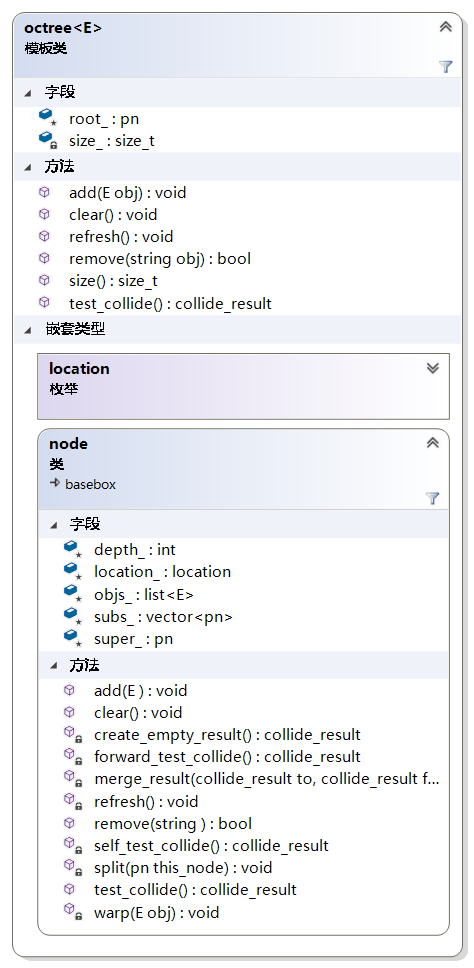
\includegraphics[width=.65\textwidth]{ClassDiagram4.png}
\caption{octree的架构} %caption是图片的标题 
\label{cd4} %此处的label相当于一个图片的专属标志,目的是方便上下文的引用 
\end{figure}

\subsection{八叉树的优化效果}
在java平台\footnote{这个结构显然不依赖于某种语言}上的一个简单测试如下表所示\footnote{测试结果平台相关}。

\begin{table}[!htbp]
    \centering
    \caption{传统方法和八叉树方法的时间对比}
    \begin{tabular}{ccc}
        \hline
        物体数量& 八叉树(ms)& 传统解法(ms)\\
        \hline
        100 & 2 & 2\\
        1000 & 5 & 19\\
        10000 & 13 & 808\\
        50000 & 33 & 42744\\
        100000 & 45 & 221641\\
        \hline
    \end{tabular}
\end{table}

可以看到这种优化方法的强大,尤其当物体的数量上涨的时候,八叉树的优势非常显著。

\section{对结果的优化}
在对方程计算的过程中,计算结果的精度是一阶的,
然而一阶的欧拉法并不是一种十分高效的计算方法,
我们可以使用更高阶的方法来对方程进行计算。
将式\ref{eular}中的一阶计算优化成四阶的Kunge-Kutta方法,
可以以增加三倍计算量为代价让结果的误差从随步长的一阶量减小到随步长的四阶量,
让计算结果的精度大幅提高。

\noindent 关于RK4方法在对此类方程求解的方程组如下:
\[ 
\left \{
\begin{array}{lr}
{\displaystyle S_{n+1} = \frac{\Delta t}{6} (k_1+2k_2+2k_3+k_4)}\\\\
{\displaystyle k_1 = f(t_n,S_n})\\\\
{\displaystyle k_2 = f(t_n+\frac{\Delta t}{2},S_n+k_1\frac{\Delta t}{2})}\\\\
{\displaystyle k_3 = f(t_n+\frac{\Delta t}{2},S_n+k_2\frac{\Delta t}{2})}\\\\
{\displaystyle k_4 = f(t_n+{\Delta t},S_n+k_3\Delta t)}
\end{array}
\right.
 \]
其中
$t_n$表示第n次迭代的时间
$S_n$表示在第n次迭代时整个场景的状态\footnote{它更像是一个帧},
$k$表示根据当前状况下的对下一状态的约束计算得到的增量

与在欧拉法的讨论中不同的是$S_n$在这个方程中的本质并不是一个简单的量,而是这个系统的状态\footnote{本质上是位形空间中的一个点集},
在这个方程的计算中,
$S_n$能线性叠加是一个关键点,
线性叠加的核心在于合适的定义对状态的加法和数乘,并使得其满足八条运算律。

我们这样定义状态的加法:两个状态的和是指对两个状态中所有相同对象的和,
对状态中对象的和定义成对象的对应量(0或1阶张量)的和。

我们这样定义状态的加法:对状态的数乘是指对状态中所有对象的数乘,
如果某个量是一个数则按照数的数乘计算,如果某个量是一个向量则按照向量的数乘计算。

显然,在增加上述定义\footnote{实际上上述定义就是对集合中每一个点的加法和数乘运算}后,状态是线性的。

使用Runge-Kutaa方法所带来的优化已经是久经考验的了,相关的文献有很多,在此不做赘述。

\section{应用举例}
%\subsection{最简单的运用——单物体单场}
一个最简单的例子是在重力场中自由下落的球
代码调用演例如下:
头文件:
{\setmainfont{Consolas}
\begin{lstlisting}
#include "kinematics_lib.h"  
class gravity_field : public field
{
public:
    explicit gravity_field(const vec3D& g) 
    : field({}, {}), g_(g){}

    bool is_in_field(double, masscenter&) override
    {
        return true;//表示全局场
    }

    void add_force(double, masscenter& obj) override
    {
        force f{gravity, g_ * obj.mass()};//f = mg
        obj.add_force(f);
    }
private:
    vec3D g_;
};
    \end{lstlisting}}\label{code_g}
源文件:
{\setmainfont{Consolas}
\begin{lstlisting}
#include "kinematics_lib.h"
#include <iostream>
int main()
{
    const masscenter mc1 =
    {"ball", {}, {1e-2, 1e-2, 1e-2}, {}, 1, 0, 0};
    const gravity_field field({0, -9.8, 0});
    physics_sence scene{};
    {
        scene.setting().delta_time = 0.01;
        scene.setting().start_time = 0;
        scene.setting().end_time = 1;
        scene.setting().save_duration = 0.2;
    }//基本设置
    scene.add_mass_center(mc1,true);//true 表示追踪
    scene.add_field(field);
    scene.run(); //计算
    const auto re = scene.get_result("ball");
    write_result(std::cout, re); //导出结果
    return 0;
}
\end{lstlisting}
}

分析最终导出的结果,我们可以看到,计算得到的结果与原结果完全符合。

\begin{figure} [bh]
    \centering 
    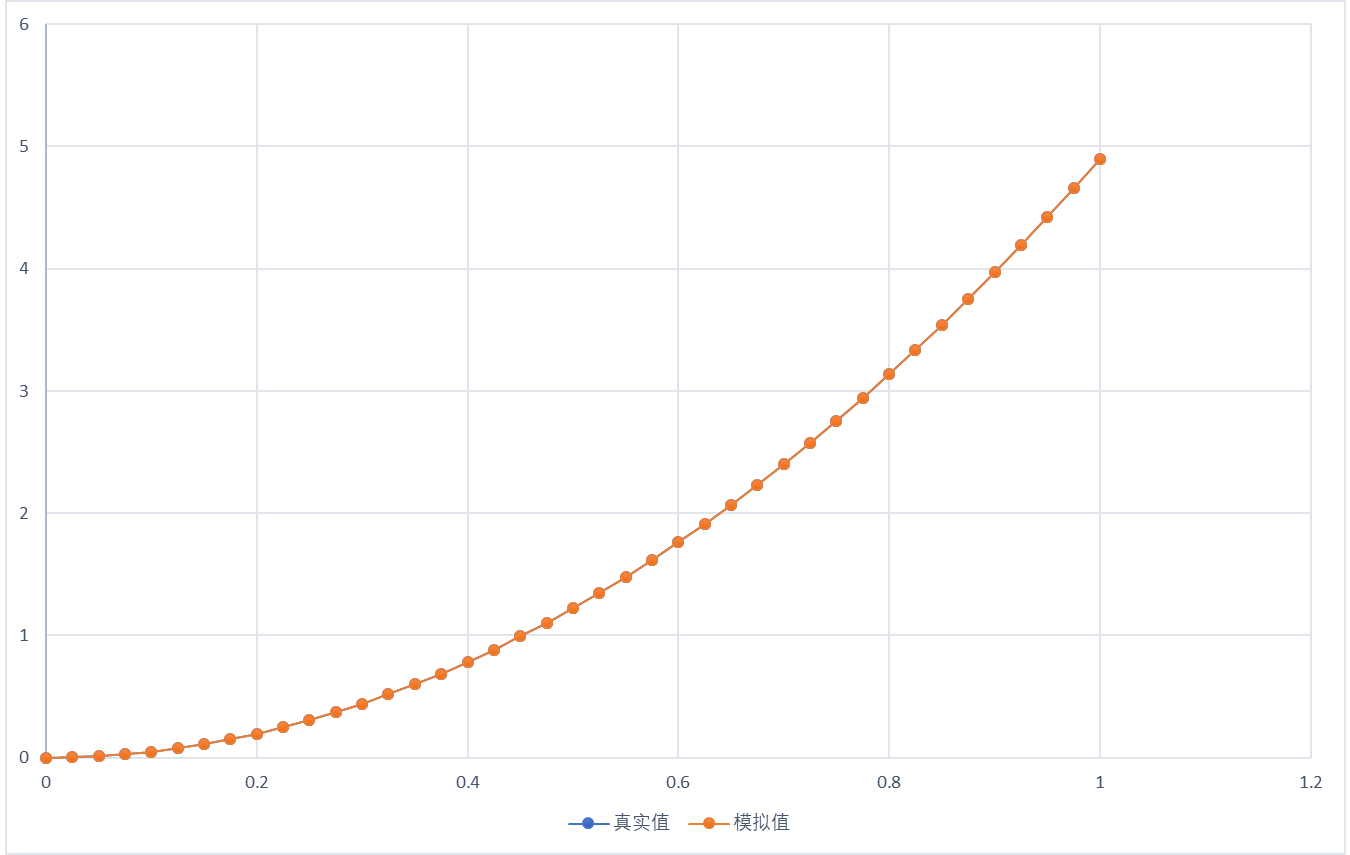
\includegraphics[width=.75\textwidth]{statics1.png}
\caption{自由落体的真实值与模拟值} 
\end{figure}

% \subsection{多体问题}
% 另一种经典的问题是多体问题,多体问题在这个框架下可以非常容易的解决,
% 如下面的展示。
%%%%%%%%%%%%%%%%%%%%%%%%%%%%
\chapter{项目优势}
\section{扩展性}
场可以被以不同的方式实现,每种实现都代表着一种场,场的性质是完全解耦的,所以对物理场的拓展性是非常好的。
以下是几种场的例子:

\noindent 首先是重力场/电场如前所述
\noindent 还可以是磁场
{\setmainfont{Consolas}
\begin{lstlisting}
class circle_magnetic_field : public field
{
public:
    circle_magnetic_field
    (const vec3D& pos, double r, const vec3D& intensity)
        : field(pos, {r, r, r})
        , intensity_(intensity)
	{
	}

	bool is_in_field(double, masscenter& obj)override
	{
        return 
        this->size().x() 
        > (this->position() - obj.position()).length();
	}

	void add_force(double, masscenter& obj) override
	{
        const auto fv =
        (obj.velocity().cross(intensity_)) 
        * obj.q();
		force f{magnetic_static, fv};
		obj.add_force(f);
	}
private:
	vec3D intensity_;
};
\end{lstlisting}
}

\noindent 再如二阶阻力场
{\setmainfont{Consolas}
\begin{lstlisting}
class reR2_field : public field
{
public:
    reR2_field(const double intensity)
        : field({},{}), intensity_(intensity)
    {
    }

    bool is_in_field(double, masscenter& obj) override
    {
        return true;
    }

    void add_force(double, masscenter& obj) override
    {
        const auto fv =obj.velocity().unit()
        *(obj.velocity()*obj.velocity())*-intensity_;
        force f{resistance, fv};
        obj.add_force(f);
    }

private:
    double intensity_;
};
\end{lstlisting}
}

\noindent 甚至是一些完全随意的场(仅供娱乐)
{\setmainfont{Consolas}
\begin{lstlisting}
class funny_field : public field
{
public:
    funny_field():field({},{}){}

    bool is_in_field(double, masscenter&)override
    {
        return rand() % 2;
    }

    void add_force(double, masscenter& obj)override
    {
        force f{extra, {rand(),rand(),rand()}};
        obj.add_force(f);
    }
};
\end{lstlisting}
}

在计算的过程中,还可以通过对物体添加事件监听器\footnote{采用监察者模式},
来完成通过简单增加场所不能解决的问题,
同时在关键性接口上留下了扩展的接口,在未来有需要的时候可以override,提高程序的复用性。
项目对拓展完全遵从开闭原则,使得整体结构有序。由于各个模块间松耦合,可以在修改时只考虑本身的业务逻辑而不会束手束脚。
这与很多用于计算的库是不同的(尤其是有些Fortan的古董库)。
\section{并行能力}
由于量子效应的存在,芯片的制程不能无限变小,可以看到在近几年计算机芯片的单核性能不能再做快速的提升,摩尔定律已经基本失效,
从提高单核性能到多核协调工作已经成为大势所趋。类似于超算的计算机可以让计算的总频率大幅提高,为了适应在大规模集群上的计算,我们在设计模型的同时考虑了
结构的并行性,并且能够在并行运行时大幅提高效率。

在这个架构中,可以并行\footnote{在本项目的源码中使用async进行实现}进行的主要有两大方面,一是帧的计算,二是内部细节的计算。

根据RK方法,我们可以依赖于具体的需求将帧的计算阶数不断提高,每提高一倍运算量就会增加一倍但是结果的精度能提高一阶,
新的帧是可以从前一帧计算得出的,我们可以采取并行化计算的方法,让每一个关键帧的下一个关键帧的计算并行,
形成$1\rightarrow n \rightarrow 1$的结构,在一个内核数目为n的计算机上,相当于通过极小的时间开销将结构的精度大幅提高。

另一方面,在每一个帧内部的计算中,我们需要进行多次遍历,而遍历的过程中许多部分都是相互独立的可以进行并行化。
对力的计算中,由于状态此时没有改变,所以每一个物理场的计算都是可以独立进行的,如果一个计算机的内核数量足够大,使得所以场的计算都是同时的,
那么施力的过程本质上就可以看作一个$O(1)$的操作。同理,碰撞检测的进行本质上依赖于的是每一个节点的计算,如果能将全部的节点同时进行计算,
时间开销也会相当小,而且碰撞和场的计算也是可以同时进行的,在这个过程中,需要等待的只有每帧最终进行的移动步骤,但是每一个移动此时也是独立的,所以仍然可以并行化处理,
整体的效率可以非常高。

综合上述两点,这个架构可以在大规模计算集群上充分的利用CPU资源,将时间大幅度压缩,同时能够提高结果的精度。
\chapter{结论}
我们提出了一种高效率高精度结构方案,可以普适的解决所有质点动力学问题,它同时具有很高的扩展性,并对大规模计算集群友好。

这个库可以在初高中物理教学、预试验、对大规模大尺度现象的模拟等方面发挥作用,有利于对物理现象的值观感受和对结果的定量分析。
高度模块化的程序既能让初学者也能轻松使用,也能让高水平用户做出拓展。可以满足各种不同的需求。

这个架构的性能仍然存有优化空间,事实上在计算的过程中,由于高阶导数的可能十分平滑,有时可以改变步长的大小加速计算,但又不会打破结果的精度要求,
我们曾经设想采取一个分支预测器来根据历史变化速率判断下一步长大小,但是这个预测很难找到一个效率与精度之间的平衡点,这是应当在未来解决的问题。

%% -*- coding: utf-8 -*-

\def\bibrangedash{ $\sim$ }
\printbibliography [ category = cited]


% -*- coding: utf-8 -*-

%\makeschapterhead{致谢}
\chapter*{致谢}
感谢郭天勇老师一学期以来的悉心教导

感谢实验室老师和助教老师的帮助

感谢全组成员三个多月来的共同学习共同努力

感谢github提供了免费的代码托管平台

感谢Bjarne Stroustrup发明了C++

感谢家长在学习生活中的关心

感谢各位室友在精神上的支持


\end{document}
